\chapter{Model Architectures for Stock Price Prediction}

\section{Overview of Proposed Architectures}

This chapter presents a comprehensive suite of model architectures and frameworks developed for stock price prediction, spanning from initial exploratory models built during the early phases of research to sophisticated hybrid and deep learning solutions designed for high accuracy and robustness. The progression reflects a systematic effort to enhance predictive performance, resolve issues such as prediction lag, and effectively leverage domain-specific knowledge through advanced feature engineering and integration techniques.

The chapter begins with a detailed description of the dataset and the preprocessing strategy adopted, including steps like data cleaning, alignment, normalization, and feature selection using statistical methods such as \textit{SelectKBest}. Feature engineering approaches to improve input signal quality and predictive power are also discussed.

Following this, various model architectures are presented:

\begin{itemize}
    \item \textbf{Hybrid LSTM-RLS Architecture:} A novel integration of LSTM for sequence modeling and Recursive Least Squares (RLS) for refining predictions.
    
    \item \textbf{Enhanced Hybrid LSTM-RLS:} A more feature-rich and modular extension, including sequence generation for RLS and multi-feature incorporation.
    
    \item \textbf{Dual Network Solution (DNS):} A parallel processing architecture designed to leverage both trend and residual components for improved performance.
    
    \item \textbf{ARIMAX-LSTM Residual Integration:} A hybrid statistical-deep learning model combining ARIMAX for linear dependencies and LSTM for capturing non-linear residual dynamics.
    
    \item \textbf{Multi-Feature LSTM Forecasting:} A deep learning framework that utilizes a broader feature set and standardized preprocessing for robust return prediction.
    
    \item \textbf{GARCH-Based Volatility Forecasting:} A statistical approach focusing on volatility modeling and its integration with deep learning architectures.
    
    \item \textbf{Stochastic Volatility with Gaussian Mixture Observations:} A custom probabilistic filtering model capturing latent volatility states using mixture distributions.
    
    \item \textbf{Custom Ensemble Learning Architecture:} An ensemble system combining multiple base learners (e.g., ARIMAX, XGBoost, CatBoost) with an LSTM-based MetaLearner to enhance generalization.
    
    \item \textbf{Transformer-based GAN for Time Series:} A generative adversarial framework incorporating Transformer encoders for sequential data generation and discrimination.
    
    \item \textbf{RAGIC Architecture:} A state of the art multi-module architecture designed for financial time series prediction, incorporating temporal modeling, attention based risk modules, and GAN-based critics.
\end{itemize}

Each architecture is accompanied by its design rationale, workflow diagrams, implementation details, training methodology, and integration strategy. Collectively, these models represent a holistic approach to modern financial time series forecasting, combining classical statistical tools, deep learning, attention mechanisms, and generative modeling.

\newpage
\section{Data Description and Preprocessing}
\subsection{Dataset Overview}
The dataset used in this study was obtained using the \texttt{yfinance} \cite{yahoo_nifty50_history} API and spans from January 1, 2014, to April 30, 2025. The primary target variable is the daily return of the NSEI index. In a few architectures, such as the DNS and Transformer-based models, the target is the close price, for which additional preprocessing was applied.

The dataset includes 12 input features:
\begin{itemize}
    \item 5, 15, 30, and 60-day returns of the open-close average
    \item 5, 15, 30, and 60-day returns of the high-low average
    \item On-Balance Volume (OBV)
    \item Relative Strength Index (RSI)
    \item Daily return of INR/USD exchange rate
    \item India Volatility Index (VIX) \cite{nse_vix}
\end{itemize}

\subsection{Data Cleaning and Alignment}
The \texttt{yfinance} data was clean and contained no missing values. For the INR/USD forex time series, values were filtered to retain only dates corresponding to valid NSEI trading days, ensuring temporal alignment across all features.

\subsection{Train-Validation-Test Split}
The data was split chronologically, preserving its sequential nature without any shuffling. The proportions for training, validation, and testing were set at 85\%, 10\%, and 5\% respectively.

\subsection{Preprocessing Strategy}
Two distinct preprocessing pipelines were followed based on the target variable:
\begin{itemize}
    \item \textbf{When the target is return-based:} No preprocessing was applied to the target or return features. These were used in their raw form to maintain interpretability.
    \item \textbf{When the target is the close price:}
    \begin{itemize}
        \item A \textbf{log transformation} was applied to reduce skewness and stabilize variance.
        \item \textbf{StandardScaler} was used to normalize the log-transformed values.
        \item A scaling factor of 2.5 was applied post-\texttt{tanh} activation to expand the output range to $[-2.5, 2.5]$.
    \end{itemize}
\end{itemize}

\begin{figure}[h]
    \centering
    \includegraphics[width=\textwidth]{Images/distribution_plot.pdf}
    \caption{Distribution plot of raw close values, log-transformed close values, and scaled log-transformed close values.}
    \label{fig:distribution_plot}
\end{figure}

\subsection{Feature Engineering Techniques}
This forecasting framework incorporates a variety of technical indicators and statistical transformations, including return-based features, RSI, OBV, and volatility indices. All input features were normalized to ensure consistency across different magnitudes and units.

The distribution of all features after normalization is depicted in Figure~\ref{fig:feature_distributions}, which illustrates their range and variability.

\begin{figure}[h!]
    \centering
    \includegraphics[width=\textwidth]{Images/feature_distributions.pdf}
    \caption{Distribution plots of all features used in the forecasting framework.}
    \label{fig:feature_distributions}
\end{figure}

The correlation matrix in Figure~\ref{fig:correlation_plot} highlights the interdependencies among the input variables and their relationships with the target variable.

\begin{figure}[h!]
    \centering
    \includegraphics[width=\textwidth]{Images/correlation_plot.pdf}
    \caption{Correlation matrix of all features in the dataset.}
    \label{fig:correlation_plot}
\end{figure}

To examine underlying temporal components of the target, a seasonal decomposition of the NSEI close price series was performed. The result, shown in Figure~\ref{fig:seasonal_decomposition}, presents the observed trend, seasonal, and residual elements.

\begin{figure}[h!]
    \centering
    \includegraphics[width=\textwidth]{Images/seasonal_decomposition.pdf}
    \caption{Seasonal decomposition of NSEI close values.}
    \label{fig:seasonal_decomposition}
\end{figure}

\subsection{Feature Selection Using SelectKBest}
To improve model efficiency and reduce overfitting, feature selection was performed using the SelectKBest method with \textsf{f\_regression}. Table~\ref{tab:feature_importance} presents the computed importance scores for each feature.

\begin{table}[h!]
\centering
\caption{Feature Importance Scores using SelectKBest}
\begin{tabular}{|l|c|}
\hline
\textbf{Feature} & \textbf{Score} \\ \hline
INDIAVIX\_1D     & 1125.250       \\ \hline
RSI\_Normalized  & 292.775        \\ \hline
Open\_Close\_5d  & 276.985        \\ \hline
High\_Low\_5d    & 268.947        \\ \hline
High\_Low\_15d   & 79.877         \\ \hline
Open\_Close\_15d & 79.634         \\ \hline
INRUSD\_X        & 42.358         \\ \hline
Open\_Close\_30d & 35.719         \\ \hline
High\_Low\_30d   & 35.260         \\ \hline
Open\_Close\_60d & 16.825         \\ \hline
High\_Low\_60d   & 16.236         \\ \hline
OBV\_Normalized  & 0.570          \\ \hline
\end{tabular}
\label{tab:feature_importance}
\end{table}

\subsection{Feature Refinement}
Features with low predictive value—such as OBV\_Normalized and long-horizon returns (30-day and 60-day)—were removed. This refinement step led to improved training efficiency and reduced model complexity, without compromising forecast accuracy.

\newpage
\section{Hybrid LSTM-RLS Architecture}

\subsection{Workflow and Design}
The Hybrid LSTM-RLS Architecture was the first model developed during my summer internship. It combines the strengths of LSTM for capturing sequential dependencies and Recursive Least Squares (RLS) for refining predictions. Figure~\ref{fig:summerarch} illustrates the architecture, highlighting the key components and their interactions.

\begin{figure}[h!]
    \centering
    \includegraphics[width=0.8\textwidth]{Images/SummerInternArchitecture.pdf} % Adjust width as needed
    \caption{Hybrid LSTM-RLS Architecture}
    \label{fig:summerarch}
\end{figure}

The workflow for this architecture is as follows:
\begin{enumerate}
    \item \textbf{Install and import libraries:} TensorFlow, NumPy, yfinance, and scikit-learn.
    \item \textbf{Fetch stock data:} Historical prices retrieved via yfinance API.
    \item \textbf{Data preprocessing:} The data was normalized, missing values were handled, and it was split into training and testing sets.
    \item \textbf{Create sequences:} Price sequences of fixed length were created as input to the LSTM model.
    \item \textbf{Train the LSTM model:} The LSTM model was trained to predict the next stock price based on these sequences.
    \item \textbf{LSTM predictions passed to RLS model:} Scalar predictions from the LSTM model were passed to the RLS model.
    \item \textbf{RLS model provides final prediction:} The RLS model used the LSTM predictions to produce refined stock price predictions.
\end{enumerate}

\section{Enhanced Hybrid LSTM-RLS Architecture}

To address issues such as dimension mismatches and long training times in the original architecture, several enhancements were implemented during Semester 3. These refinements simplified the process and improved predictive accuracy.

Figure~\ref{fig:Refinedarch} illustrates the improved workflow. The modifications made the architecture more efficient and straightforward for stock price forecasting.

\subsection{Architecture Workflow}

\begin{figure}[htbp]
    \centering
    \includegraphics[width=0.8\textwidth]{Images/RefinedArchitecture.pdf} % Replace with the actual image file
    \caption{Enhanced Hybrid LSTM-RLS Architecture}
    \label{fig:Refinedarch}
\end{figure}

The architecture process involves the following steps:

\begin{enumerate}
    \item \textbf{Install and import necessary libraries:}
    \begin{itemize}
        \item Libraries such as \texttt{yfinance}, \texttt{tensorflow}, \texttt{scikit-learn}, and others were imported.
    \end{itemize}
    
    \item \textbf{Import Nifty 50 daily close price data:}
    \begin{itemize}
        \item Closing prices of the Nifty 50 index for the last 12 years were fetched daily using the \texttt{yfinance} API.
    \end{itemize}
    
    \item \textbf{Normalize the data:}
    \begin{itemize}
        \item Data normalized to [0, 1] using \texttt{MinMaxScaler}.
    \end{itemize}
    
    \item \textbf{Sequence creation for LSTM:}
    \begin{itemize}
        \item Sequences of historical stock prices were created as inputs for training the LSTM \cite{staudemeyer_understanding_2019} model.
    \end{itemize}
    
    \item \textbf{Split dataset into training and testing set}
    \begin{itemize}
        \item The sequences were divided into training (80\%) and testing (20\%) sets to evaluate model performance.
    \end{itemize}
    
    \item \textbf{Training of the LSTM model:}
    \begin{itemize}
        \item The LSTM model was trained on the 80\% training data over several epochs to predict stock prices.
    \end{itemize}
    
    \item \textbf{Input Sequences creation for RLS:}
    \begin{itemize}
        \item Predictions from the LSTM model is used to prepare input sequences for the RLS model.
    \end{itemize}
    
    \item \textbf{Forecast Stock Prices with RLS:}
    \begin{itemize}
        \item The RLS model processed the LSTM predictions as inputs, producing the final stock price forecasts.
    \end{itemize}
    
\end{enumerate}

\subsection{Developing Input Sequences for RLS}

Figure~\ref{fig:inputseq} provides a detailed view of the sequence development process for the RLS model based on LSTM predictions.

\begin{figure}[htbp]
    \centering
    \includegraphics[width=0.8\textwidth]{Images/RLSInputCreation.pdf} % Replace with the actual image file
    \caption{Input Sequence Formation for RLS}
    \label{fig:inputseq}
\end{figure}

The following steps outline the process:

\begin{enumerate}
    \item \textbf{Original Sequence for LSTM:}
    \begin{itemize}
        \item The original sequence of stock prices served as the input for training the LSTM model.
        \item For example, a sequence ranging from index 0 to 49 was selected.
    \end{itemize}
    
    \item \textbf{Training the LSTM Model:}
    \begin{itemize}
        \item The LSTM model was trained on the input sequence.
        \item Upon training, the model predicted the 50th value based on the prior 49 values.
    \end{itemize}
    
    \item \textbf{Shifting the Sequence for RLS Input:}
    \begin{itemize}
        \item The sequence was shifted by one step to generate input for the RLS model.
        \item For instance, the updated sequence started at index 1 and extended to index 50, incorporating the LSTM prediction for the 50th point.
    \end{itemize}
    
    \item \textbf{Final Input for RLS Model:}
    \begin{itemize}
        \item The shifted sequence (from index 1 to 50) was provided as input to the RLS model.
        \item The RLS model used this sequence to produce the final stock price prediction.
    \end{itemize}
\end{enumerate}

This sliding window approach facilitated seamless integration between the LSTM and RLS models, ensuring improved accuracy and efficient stock price forecasting.

\subsection{Multi-Feature Hybrid LSTM-RLS Implementation}

The preprocessed dataset was directly used in the \textbf{Hybrid LSTM-RLS architecture}. See \textbf{Figure~\ref{fig:HybridLSTM_RLS_M}} for the workflow.

\begin{figure}[h!]
    \centering
    \includegraphics[width=0.8\textwidth]{Images/HybridLSTM_RLS_M.pdf}
    \caption{Flow diagram of Multi-Feature Hybrid LSTM-RLS implementation.}
    \label{fig:HybridLSTM_RLS_M}
\end{figure}

The LSTM model was trained following the standard sequence based approach, where multi-feature input sequences were constructed and used for training.

\subsubsection{Key Modification: RLS Input Sequence Construction}

A significant deviation from the previous approach was the method used to construct input sequences for the \textbf{Recursive Least Squares (RLS) model}. As illustrated in \textbf{Figure~\ref{fig:RLS_Input_M}}, the input sequence creation for RLS followed a structured pipeline:

\begin{figure}[h!]
    \centering
    \includegraphics[width=0.8\textwidth]{Images/RLS_Input_M.pdf}
    \caption{RLS input sequence construction using LSTM outputs.}
    \label{fig:RLS_Input_M}
\end{figure}

\begin{itemize}
    \item Instead of deriving the RLS input sequences from the \textbf{LSTM input sequence}, the sequences were generated using \textbf{returns and close prices}.  
    \item The LSTM model was trained on sequences created from the \textbf{multi-feature input} (\textbf{X}). Once trained, the predicted values from LSTM were appended to the sequences constructed from \textbf{daily returns} (\textbf{Y}), ensuring that the RLS model receives inputs of the same nature as its output, thus allowing effective prediction in an online setting.
    \item Two separate training strategies were employed:  
    \begin{itemize}
        \item \textbf{Predicting Returns}: The model was trained to forecast stock returns, leveraging the structured relationship between past returns and future movements.  
        \item \textbf{Predicting Close Prices}: The model was also trained using close prices to evaluate its performance in direct price prediction.
    \end{itemize}
\end{itemize}

\subsubsection{Impact of this Approach}

\begin{itemize}
    \item \textbf{Alternative Feature Representation}: By constructing input sequences \\from returns and close prices, the model captured different aspects of market behavior.  
    \item \textbf{Comparative Performance Analysis}: Training for both returns and close prices allowed an in-depth evaluation of prediction effectiveness under different target variable choices.  
    \item \textbf{Flexible RLS Adaptation}: The RLS model benefited from this new input structure, enabling it to adjust dynamically to either return-based or price-based forecasts.  
\end{itemize}

This modification provided insights into how input sequence construction affects the overall model accuracy and adaptability, further refining the \textbf{Hybrid LSTM-RLS architecture}.

\section{Dual Network Solution (DNS) Architecture}
\subsection{Design and Integration}
The Dual Network Solution (DNS) architecture addresses the one-time-step lag observed in the previous models. Figure~\ref{fig:DNSArch} shows the DNS architecture, which involves two networks: one trained on trends and the other on actual data.

\begin{figure}[h!]
    \centering
    \includegraphics[width=0.8\textwidth]{Images/DNSArchitecture.pdf} % Adjust width as needed
    \caption{DNS Architecture}
    \label{fig:DNSArch}
\end{figure}

Steps include:
\begin{enumerate}
    \item \textbf{Trend extraction:} Network 1 is trained to predict trends using slope differences or moving averages.
    \item \textbf{Prediction refinement:} Network 2 uses the output of Network 1 to generate lag-free predictions.
\end{enumerate}

% \section{Advanced Data Preprocessing for Enhanced\\ Model Performance}
% \subsection{Challenges in Scaling and Activation}
% During the development of the stock price prediction models, challenges arose when scaling the data using traditional normalization techniques such as MinMaxScaler. This approach limits the range of predictions to the maximum value observed during training, potentially capping future predictions. To address this issue, an alternative preprocessing technique was introduced, which involves:
% \begin{itemize}
%     \item \textbf{Log Transformation:} Applying a logarithmic transformation to the close price values to reduce large variations and stabilize the data.
%     \item \textbf{Standardization:} Standardizing the log-transformed values to ensure that the data is centered and scaled, allowing it to be processed effectively by the model.
% \end{itemize}

% After preprocessing, the resulting data ranged approximately between $-2$ and $2$. To handle this range, the \texttt{tanh} activation function was selected for its natural prediction range of $[-1, 1]$. However, to ensure flexibility in predictions beyond this range:
% \begin{itemize}
%     \item A multiplier of $2.5$ was applied after the \texttt{tanh} activation function. This adjustment extended the prediction range to $[-2.5, 2.5]$, providing additional room for extreme values without capping predictions.
% \end{itemize}

% Figure~\ref{fig:distribution_plot} shows the distribution plot of the raw close values, log-transformed close values, and scaled log-transformed values. This plot depicts how the preprocessing steps have allowed the data to fall in a range that the activation function can handle effectively.

% \begin{figure}[h]
%     \centering
%     \includegraphics[width=\textwidth]{Images/distribution_plot.pdf}
%     \caption{Distribution plot of raw close values, log-transformed close values, and scaled log-transformed close values.}
%     \label{fig:distribution_plot}
% \end{figure}

% \subsection{Application in DNS Architecture}
% This preprocessing technique, as explained in Section 3.5.1 was used in the concept of the Dual Network Solution Architecture. Using log transformation, standardization, and modified range of activation functions,
% the DNS model represents both linear and nonlinear parts of
% stock price movements.

% This preprocess step was crucial in enhancing the prediction accuracy of the model.
% racy of the DNS architecture, so that it could support a greater number of values
% While the predictions of strength were retained, the changes had provided the basis for
% groundwork for subsequent enhancements in model design and integration.

\section{ARIMAX-LSTM Residual Integration Framework}
\subsection{ARIMAX-LSTM Hybridization}

The initial approach involved integrating the capability of ARIMA to model linear patterns and LSTM's strength in capturing non-linear relationships. However, due to suboptimal performance, the ARIMA model was replaced with ARIMAX \cite{9998301} for handling the linear component while LSTM continued to process residuals. The final prediction was obtained by integrating the outputs of these two models. The revised framework consists of:

\begin{itemize}
    \item \textbf{ARIMAX model for linear trends:} Unlike ARIMA, ARIMAX incorporates external features alongside past values to better capture the linear component of stock prices.
    \item \textbf{LSTM model for residuals:} LSTM models the remaining non-linear residuals after ARIMAX processing.
    \item \textbf{Final integration:} Predictions from both models are combined to enhance accuracy.
\end{itemize}

\subsection{Challenges and Model Refinement}

Initially, the ARIMA-LSTM hybrid model was tested; however, its performance was unsatisfactory. The residuals did not capture sufficient differences between the original close price values and ARIMA’s linear predictions, leading to subpar results. 

To address this issue:
\begin{itemize}
    \item The \textbf{ARIMA model was replaced with ARIMAX}, incorporating external variables to improve the modeling of linear relationships.
    \item The \textbf{LSTM model remained responsible for capturing non-linear residuals}.
    \item The integration of \textbf{ARIMAX and LSTM} was evaluated to determine if this modification led to improved performance.
\end{itemize}

This refined framework aimed to leverage ARIMAX's enhanced linear modeling alongside LSTM's capacity for non-linearity, ultimately improving the predictive capability of the model.

\subsection{Applying RLS to Residuals Framework Output}

In the \textbf{ARIMAX-LSTM-RLS model}, after predicting returns using the \textbf{ARIMA-LSTM Residual Integration Framework}, the next step involved incorporating \textbf{Recursive Least Squares (RLS)} to refine the final predictions.

\subsubsection{RLS Input Sequence Construction}

To enhance the prediction accuracy, input sequences for RLS were constructed as follows:
\begin{itemize}
    \item The predicted returns obtained from the \textbf{residuals architecture} were used to generate input sequences for RLS.
    \item RLS was then applied to these sequences, providing the \textbf{final predicted returns output}.
\end{itemize}

\subsubsection{Impact of RLS on the Residuals Architecture}

\begin{itemize}
    \item \textbf{Sequential Refinement}: By feeding the residuals architecture's output into RLS, the model aimed to further refine the predictions.
    \item \textbf{Performance Evaluation}: The final output from RLS was analyzed to determine whether this additional step improved the overall prediction accuracy.
\end{itemize}

This integration of RLS with the residuals architecture provided valuable insights into whether the additional layer of processing contributed to enhanced model performance.

\section{Multi-Feature LSTM Forecasting Framework}
\subsection{Overview and Objectives}
The Multi-Feature LSTM Forecasting Framework aims to enhance stock price prediction accuracy by incorporating a diverse set of features derived from technical indicators and price patterns. These features include daily returns, Relative Strength Index (RSI), On-Balance Volume (OBV), and various ratios capturing short-term and long-term price movements. 

The key objectives of this framework are:
\begin{itemize}
    \item Many key features for an integrated understanding of
Market Behavior.
    \item Developing a methodology of training that is robust and adaptive for daily usage.
    \item It uses the strength of LSTM in capturing temporal dependency.
cies within financial data.
\end{itemize}

The framework is designed based on the model's adaptability with respect to newer ideas. Market trend with scalability and computational effectiveness of a solution.
Incorporation of feature selection and refinement adds further sophistication to the predictivity ability of the model.

\subsection{Training Methodology}
This is specific for the Multi-Feature LSTM Forecasting Framework. Designed for high-level real-time stock market information processing and daily changes. The methodology involved the following:
\subsubsection{One-Step Prediction and Incremental Training}
That makes the prediction of the stock price at the next step a function of only
Minimize the error between the predicted and actual values for the immediate next day. Even though it is predicting several future time steps, only the first
The predicted value is used in the context of algorithmic trading for decision making.
Immediately after obtaining tomorrow's true value, the training and testing datasets
are updated:
\begin{enumerate}
    \item Function that omits the first value in the training dataset and the last value from the test dataset is appended to keep the no of training sample sizes.
    \item The first value in the test data set is removed, and the newly
real value is returned by the final entry of available.
\end{enumerate}

This means the model is updated on the most recently available data points.
It enables it to adjust to changes in the market. The model is trained daily
With such an updated dataset, predictions of the following day can be made

\subsubsection{Visualization of Incremental Training Process}
The incremental training process is visualized in Figure~\ref{fig:incremental_training}. This figure illustrates the dynamic updates to the training and testing datasets as new data becomes available. The real-time adaptability of the model is a key feature that supports its application in live trading environments.

\begin{figure}[h!]
    \centering
    \includegraphics[width=\textwidth]{Images/incremental_training.pdf}
    \caption{Visualization of the Incremental Training Process for Multi-Feature LSTM Forecasting Framework.}
    \label{fig:incremental_training}
\end{figure}

% \subsection{Feature Engineering Techniques}
% This framework incorporates multiple features, such as returns, RSI, and OBV, to enhance predictive accuracy. All features were normalized for consistency. 

% The distribution of all features in the dataset is shown in Figure~\ref{fig:feature_distributions}. This plot highlights the range and variability of each feature, demonstrating the effectiveness of normalization.

% \begin{figure}[h!]
%     \centering
%     \includegraphics[width=\textwidth]{Images/feature_distributions.pdf}
%     \caption{Distribution plots of all features used in the forecasting framework.}
%     \label{fig:feature_distributions}
% \end{figure}

% Additionally, the correlation matrix for all features is displayed in Figure~\ref{fig:correlation_plot}. This plot provides insights into feature interdependencies and the strength of their relationships with the target variable.

% \begin{figure}[h!]
%     \centering
%     \includegraphics[width=\textwidth]{Images/correlation_plot.pdf}
%     \caption{Correlation matrix of all features in the dataset.}
%     \label{fig:correlation_plot}
% \end{figure}

% Finally, Figure~\ref{fig:seasonal_decomposition} presents the seasonal decomposition plot of NSEI close values, illustrating the observed trend, seasonality, and residual components. This visualization assists in understanding the underlying temporal patterns of the target variable.

% \begin{figure}[h!]
%     \centering
%     \includegraphics[width=\textwidth]{Images/seasonal_decomposition.pdf}
%     \caption{Seasonal decomposition of NSEI close values.}
%     \label{fig:seasonal_decomposition}
% \end{figure}

% \subsection{Feature Selection Using SelectKBest}
% Feature selection was performed using the SelectKBest method with \textsf{f\_regression}. The feature importance scores are presented in Table~\ref{tab:feature_importance}.

% \begin{table}[h!]
% \centering
% \caption{Feature Importance Scores using SelectKBest}
% \begin{tabular}{|l|c|}
% \hline
% \textbf{Feature} & \textbf{Score} \\ \hline
% INDIAVIX\_1D     & 1125.250181    \\ \hline
% RSI\_Normalized  & 292.775295     \\ \hline
% Open\_Close\_5d  & 276.984547     \\ \hline
% High\_Low\_5d    & 268.947328     \\ \hline
% High\_Low\_15d   & 79.876745      \\ \hline
% Open\_Close\_15d & 79.634278      \\ \hline
% INRUSD\_X        & 42.357608      \\ \hline
% Open\_Close\_30d & 35.719346      \\ \hline
% High\_Low\_30d   & 35.259659      \\ \hline
% Open\_Close\_60d & 16.824506      \\ \hline
% High\_Low\_60d   & 16.235917      \\ \hline
% OBV\_Normalized  & 0.570088       \\ \hline
% \end{tabular}

% \label{tab:feature_importance}
% \end{table}

% \subsection{Feature Refinement}
% Low-importance features such as OBV\_Normalized and 30-day/60-day returns were dropped. The refined feature set ensured better model performance with reduced complexity.

\newpage
\section{GARCH for Stock Price Prediction}

\subsection{Introduction to GARCH}

The Generalized Autoregressive Conditional Heteroskedasticity (GARCH) \cite{BOLLERSLEV1986307} model is widely used in financial time series modeling due to its ability to capture volatility clustering. In stock markets, volatility tends to persist over time, meaning that periods of high volatility are often followed by more volatile periods, and similarly for low volatility. Since the target variable in this study is \textbf{daily returns}, which inherently exhibits volatility characteristics, GARCH is a suitable choice for modeling this behavior.

GARCH is particularly relevant to this study because it models conditional variance, providing insights into future uncertainty levels. By leveraging GARCH, we aim to enhance stock return prediction by explicitly modeling the variance dynamics, which traditional models might overlook.

\subsection{Model Implementation}

To implement GARCH, the following approach was used:

\begin{itemize}
    \item \textbf{Mean Prediction using ARIMAX:} Before applying GARCH, the mean component of stock returns was modeled using the ARIMAX model. ARIMAX extends ARIMA by incorporating external regressors, making it suitable for capturing linear dependencies in stock returns.
    \item \textbf{Residuals Extraction:} After obtaining the ARIMAX predictions, the residuals (unexplained variations) were extracted. These residuals capture the unpredictable fluctuations in returns.
    \item \textbf{GARCH Modeling on Residuals:} The extracted residuals were then used to train a GARCH model, which estimated the conditional variance of the returns. The GARCH model accounted for volatility clustering, ensuring that periods of high variance were correctly modeled.
\end{itemize}

\subsection{Integration with Existing Architectures}

The GARCH model was not used in isolation but was integrated into the broader framework of stock price prediction. Specifically:

\begin{itemize}
    \item The \textbf{ARIMAX model} was used for predicting the mean returns.
    \item The \textbf{GARCH model} was applied to the residuals from ARIMAX to model volatility.
    \item The final output was a combination of the ARIMAX-predicted mean and the variance estimation from the GARCH model, providing a more comprehensive prediction of stock returns.
\end{itemize}

By integrating GARCH with ARIMAX, the model was able to separately handle both the trend and volatility components of stock returns, improving the overall robustness of the forecasting framework.

\section{Stochastic Volatility Model with Gaussian Mixture Observation}
\label{sec:sv-model}

\subsection{Model Specification}

The stochastic volatility (SV) model describes the evolution of the latent log-volatility $x_t$ as an autoregressive process:

\begin{equation}
x_t = \phi_0 + \phi_1 x_{t-1} + \eta_t, \quad \eta_t \sim \mathcal{N}(0, \sigma_Q^2)
\end{equation}

The observation equation is modeled as a two-component Gaussian mixture:

\begin{equation}
y_t \sim 0.5 \cdot \mathcal{N}(0, e^{x_t} + \sigma_{R0}^2) + 0.5 \cdot \mathcal{N}(\mu_1, e^{x_t} + \sigma_{R1}^2)
\end{equation}

This mixture structure allows the model to capture heavy tails in financial return distributions, where $y_t = \log(r_t^2 + \varepsilon)$ represents the log-squared normalized return with a small constant $\varepsilon$ to avoid numerical instability.

\subsection{Filtering Procedure}

We implement a recursive filtering algorithm to estimate the hidden state $x_t$ at each time step:

\begin{enumerate}
    \item \textbf{Prediction:}
    \begin{align}
        x_t^- &= \phi_0 + \phi_1 x_{t-1} \\
        P_t^- &= \phi_1^2 P_{t-1} + \sigma_Q^2
    \end{align}
    
    \item \textbf{Compute Likelihoods:}
    \begin{align}
        p_0 &= \mathcal{N}(y_t; 0, e^{x_t^-} + \sigma_{R0}^2) \\
        p_1 &= \mathcal{N}(y_t; \mu_1, e^{x_t^-} + \sigma_{R1}^2)
    \end{align}
    
    \item \textbf{Posterior Weights:}
    \begin{align}
        w_0 &= \frac{0.5 \cdot p_0}{0.5 \cdot p_0 + 0.5 \cdot p_1}, \quad w_1 = 1 - w_0
    \end{align}
    
    \item \textbf{Update:}
    \begin{align}
        \text{residual} &= w_0 \cdot \frac{y_t - 0}{\text{var}_0} + w_1 \cdot \frac{y_t - \mu_1}{\text{var}_1} \\
        \text{gain} &= \frac{P_t^-}{P_t^- + w_0 \cdot \text{var}_0 + w_1 \cdot \text{var}_1} \\
        x_t &= x_t^- + \text{gain} \cdot \text{residual}
    \end{align}
\end{enumerate}

This Kalman-like update allows efficient recursive estimation of the latent volatility under the non-Gaussian observation framework.

\subsection{Parameter Estimation}

Model parameters are estimated by minimizing the negative log-likelihood of the entire sequence using the L-BFGS-B optimization algorithm, subject to bounds ensuring stationarity and numerical stability.

% \clearpage
% \appendix
% \section{Estimated Parameters for the Stochastic Volatility Model}
% \label{appendix:sv-params}

% \begin{table}[H]
% \centering
% \caption{Final Estimated Parameters and Standard Errors}
% \begin{tabular}{lcc}
% \toprule
% \textbf{Parameter} & \textbf{Estimate} & \textbf{Standard Error} \\
% \midrule
% $\phi_0$     & -0.2673  & 0.7626  \\
% $\phi_1$     & 0.8644   & 0.5623  \\
% $\sigma_Q$   & 5.0000   & 37.8893 \\
% $\alpha$     & 0.9361   & 14.5753 \\
% $\sigma_{R0}$ & 1.0566  & 0.8037  \\
% $\mu_1$      & -3.1405  & 0.8446  \\
% $\sigma_{R1}$ & 2.2621  & 0.5529  \\
% \bottomrule
% \end{tabular}
% \end{table}


\section{Custom Ensemble Learning Architecture}

\subsection{Theory and Architecture Overview}

This model is an ensemble learning framework designed to improve predictive accuracy by combining multiple base regressors and modeling their outputs using a neural network-based MetaLearner. The architecture consists of:

\begin{enumerate}
    \item \textbf{Base Models:} Four tree-based regressors (XGBoost, LightGBM, CatBoost, RandomForest \cite{breiman2001random}) and a time series model (ARIMAX).
    \item \textbf{Meta Feature Generator:} Uses predictions from base models and their rolling MAE to construct meta features.
    \item \textbf{MetaLearner:} A sequence-based LSTM model that learns to optimally combine meta features to predict the final target.
\end{enumerate}

The ensemble leverages the strengths of both:
\begin{itemize}
    \item \textit{Tree-based models} for capturing nonlinear patterns.
    \item \textit{ARIMAX} for linear autoregressive temporal relationships.
    \item \textit{LSTM} for modeling sequential dependence in prediction errors and combining predictions dynamically.
\end{itemize}

\subsection{Meta Feature Representation}

Each input $\mathbf{x}_t \in \mathbb{R}^{d}$ is passed to the base models and ARIMAX to produce scalar predictions $\hat{y}_{t}^{(i)}$ for each model $i$. Along with each prediction, a rolling MAE score is computed:

\begin{equation}
\text{MAE}_{t}^{(i)} = \frac{1}{w} \sum_{j=t-w+1}^{t} \left| y_j - \hat{y}_j^{(i)} \right|
\end{equation}

The meta input $\mathbf{z}_t \in \mathbb{R}^{5 \times 2}$ at time $t$ is constructed as:

\begin{equation}
\mathbf{z}_t = \left[ \left( \hat{y}_t^{(i)}, \text{MAE}_t^{(i)} \right) \right]_{i=1}^5
\end{equation}

where $i = \{ \text{XGB, LGB, CAT, RF, ARIMAX} \}$.

\subsection{MetaLearner Model}

The MetaLearner is a neural network consisting of:
\begin{itemize}
    \item \textbf{Input:} Sequence of shape $(5, 2)$
    \item \textbf{LSTM Layer:} 16 units with ReLU activation
    \item \textbf{Dense Output Layer:} Single scalar prediction
\end{itemize}

The output of the MetaLearner is given by:

\begin{equation}
\hat{y}_t^{\text{meta}} = \text{Dense} \left( \text{LSTM}(\mathbf{z}_t) \right)
\end{equation}

\subsection{Algorithm Flow}

\begin{enumerate}
    \item \textbf{Load and Split Dataset} into train, validation, and test sets.
    \item \textbf{Train Base Models:}
    \begin{itemize}
        \item XGBoost
        \item LightGBM
        \item CatBoost
        \item RandomForest
        \item ARIMAX (on training set)
    \end{itemize}
    \item \textbf{Generate Meta Features:}
    \begin{itemize}
        \item For each time step in train/val/test:
        \begin{itemize}
            \item Predict using each base model
            \item Forecast ARIMAX
            \item Calculate rolling MAE of each model
            \item Store $(\text{prediction}, \text{MAE})$ as meta feature
        \end{itemize}
    \end{itemize}
    \item \textbf{Train MetaLearner (LSTM):}
    \begin{itemize}
        \item Input: meta feature sequence $(5, 2)$
        \item Output: predicted value $\hat{y}_t$
    \end{itemize}
    \item \textbf{Evaluate on Validation and Test Set} using RMSE
\end{enumerate}

% \subsection{Pseudocode}

% \begin{verbatim}
% Function CustomEnsembleLearningModel(X_train, y_train, X_val, y_val, X_test, y_test):
%     Step 1: Train base models (XGB, LGB, CAT, RF)
%     Step 2: Fit ARIMAX on y_train with X_train as exog
%     Step 3: For each sample in train/val/test:
%         - Predict using all base models
%         - Forecast ARIMAX
%         - Compute rolling MAE for each model
%         - Store [prediction, MAE] as meta feature
%     Step 4: Stack meta features into 3D array of shape (N, 5, 2)
%     Step 5: Build and train LSTM model on meta features
%     Step 6: Predict on validation and test meta features
%     Step 7: Compute and log RMSE for all models and MetaNet

% End Function
% \end{verbatim}

\section{Transformer-based GAN Architecture}

In this section, we propose a sequence-to-one forecasting framework inspired by the TTS-GAN architecture as proposed in \cite{yoon_time-series_2019}. The model consists of a Generator and a Discriminator, both built using Transformer Encoder blocks to effectively process multivariate sequential data. The architecture leverages self-attention mechanisms to capture temporal dependencies and contextual relationships across multiple input features.

The Generator takes a fixed-length historical input sequence and outputs a single predicted return value for the next time step. The Discriminator, in turn, distinguishes between the real future value and the one generated by the Generator, thereby adversarially training the system to enhance the quality and realism of predictions.

This Transformer-based GAN approach enables more robust modeling of complex nonlinear patterns in financial time series data and shows promise in generating plausible and sharp return estimates for short-term stock price prediction.
\subsection{Generator Architecture}

The Generator $G$ takes as input a multivariate sequence $X \in \mathbb{R}^{T \times d}$ of length $T=60$ with $d=12$ features and predicts a scalar output $\hat{y}_{t+1} \in \mathbb{R}$. The input is first linearly projected into an embedding space and combined with learned positional encodings:
\[
x'_t = \text{Dense}(X_t) + \text{Embedding}(t)
\]
This representation is passed through $L$ stacked Transformer Encoder blocks, followed by a Global Average Pooling operation and a final dense layer:
\[
\hat{y}_{t+1} = G(X) = \text{Dense}(\text{GAP}(\text{TransformerBlocks}(x')))
\]

\subsection{Discriminator Architecture}

The Discriminator $D$ takes as input a univariate sequence of length 61: a real or generated scalar return $\hat{y}_{t+1}$ appended to the past 60 true values $y_{t-59}, \dots, y_t$. The architecture is similar to the Generator: a dense projection followed by positional embeddings and multiple Transformer blocks. The final output is a scalar in $[0, 1]$:
\[
D(Z) = \sigma(\text{Dense}(\text{GAP}(\text{TransformerBlocks}(Z))))
\]
where $Z \in \mathbb{R}^{61 \times 1}$ is the sequence and $\sigma$ denotes the sigmoid activation.

\subsection{Transformer Encoder Block}

\begingroup
\sloppy
Each Transformer Encoder block consists of a Multi-Head Self-Attention (MHSA) layer followed by a feed-forward network (FFN):
\endgroup

\[
\text{MHSA}(X) = \text{LayerNorm}(X + \text{Dropout}(\text{MultiHeadAttention}(X, X)))
\]
\[
\text{FFN}(X) = \text{LayerNorm}(\text{MHSA}(X) + \text{Dropout}(\text{Dense}(\text{GELU}(\text{Dense}(X)))))
\]

\subsection{Training Procedure}

The model is trained using a combination of mean squared error (MSE) and adversarial loss. Let $y_{t+1}$ be the true target and $\hat{y}_{t+1}$ the generator's prediction. The Discriminator loss is given by:
\[
\mathcal{L}_D = \text{BCE}(1, D(y_{\text{seq}}^{\text{real}})) + \text{BCE}(0, D(y_{\text{seq}}^{\text{fake}}))
\]
where $y_{\text{seq}}^{\text{real}} = [y_{t-59}, \dots, y_t, y_{t+1}]$ and $y_{\text{seq}}^{\text{fake}} = [y_{t-59}, \dots, y_t, \hat{y}_{t+1}]$.

The Generator is optimized using:
\[
\mathcal{L}_G = \text{MSE}(y_{t+1}, \hat{y}_{t+1}) + \lambda \cdot \text{BCE}(1, D(y_{\text{seq}}^{\text{fake}}))
\]
where $\lambda$ is a small weighting factor for adversarial loss (e.g., $\lambda = 0.01$).

\subsection{Optimization}

Gradients are computed using backpropagation through both the Generator and Discriminator. Separate optimizers are used for $G$ and $D$, and their parameters are updated iteratively at each training step.

\newpage
\section{RAGIC Architecture for Financial Time Series Forecasting}

\subsection{Overview}

The \textbf{RAGIC (Risk-Aware Generator with Integrated Critic)} architecture is a hybrid deep learning framework developed to model financial time series data with enhanced robustness and generalization. It integrates noise-injected attention mechanisms, temporal modeling using multi-head attention and TCNs, and adversarial learning using a Wasserstein critic to improve prediction performance on volatile data.

RAGIC is designed to forecast the next value in a sequence (e.g., stock return or price) by conditioning on multivariate historical data. It consists of three main modules:
\begin{itemize}
    \item \textbf{Risk Module} (attention + noise for uncertainty modeling)
    \item \textbf{Temporal Module} (Transformer + TCN for time series understanding)
    \item \textbf{Critic} (Wasserstein GAN discriminator to enforce realistic prediction quality)
\end{itemize}

\begin{figure}[H]
    \centering
    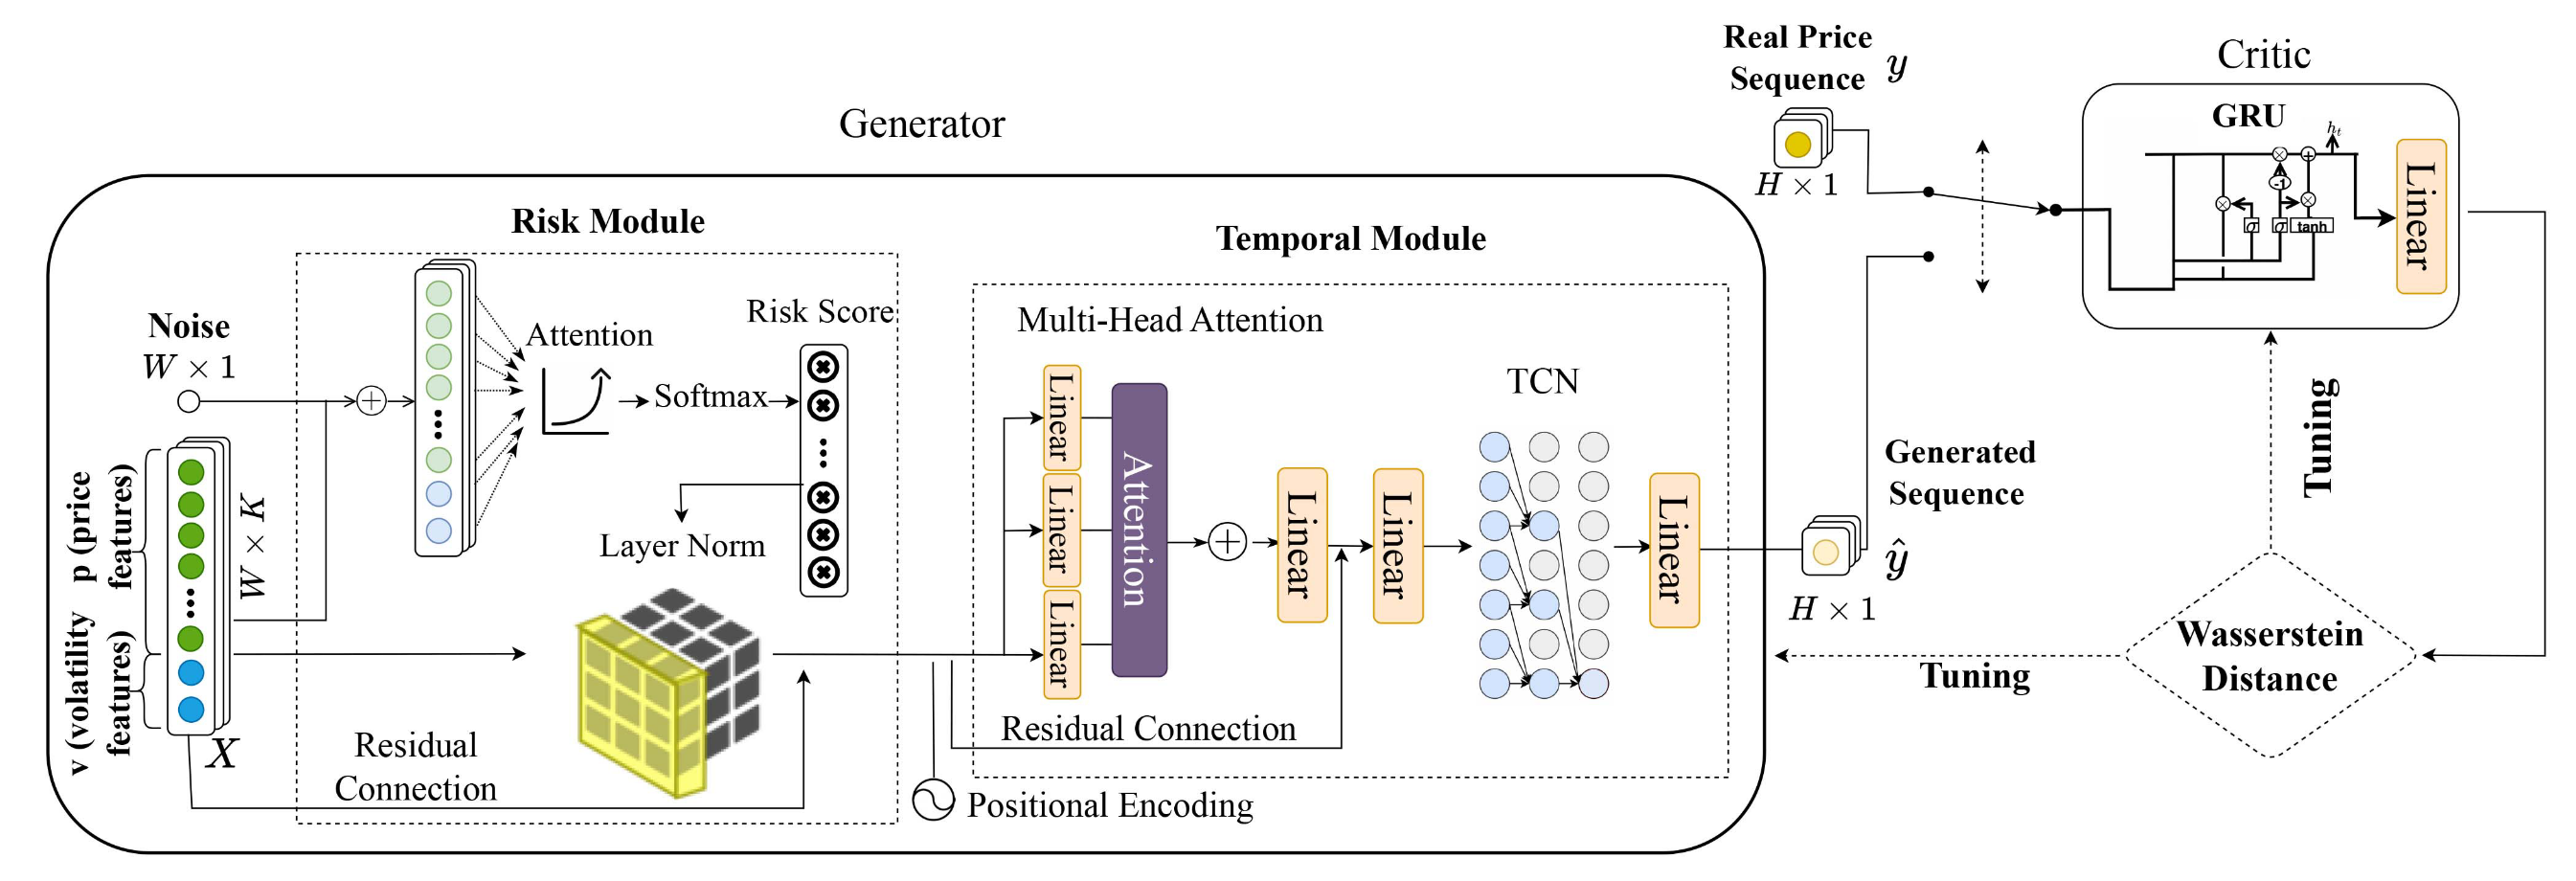
\includegraphics[width=0.95\textwidth]{Images/Screenshot 2025-05-19 at 15.00.48.png}
    \caption{RAGIC Architecture diagram \cite{gu_ragic_2025}.}
    \label{fig:ragic_architecture}
\end{figure}
The overall architecture of RAGIC, including its three key modules and data flow, is illustrated in Figure~\ref{fig:ragic_architecture}.

\subsection{Theory and Components}

\subsubsection{Risk Module}

The \textbf{Risk Module} aims to model market uncertainty by injecting Gaussian noise into the input sequence and applying attention-based weighting. This mechanism allows the model to focus on uncertain and potentially volatile patterns.

Given input $X \in \mathbb{R}^{W \times K}$ and noise $\epsilon \sim \mathcal{N}(0, I)$ of shape $\mathbb{R}^{W \times 1}$, the steps are:
\begin{enumerate}
    \item Concatenate: $X_{\text{aug}} = [X \, | \, \epsilon]$
    \item Attention weights: $a = \text{softmax}(WX_{\text{aug}})$
    \item Weighted input: $\tilde{X} = a \odot X$
    \item Residual connection and normalization: $X_{\text{risk}} = \text{LayerNorm}(\tilde{X} + X)$
\end{enumerate}

\subsubsection{Temporal Module}

The \textbf{Temporal Module} processes the output of the risk module through a combination of positional embeddings, multi-head self-attention, and a two-layer Temporal Convolutional Network (TCN). It captures both long-term dependencies and local temporal dynamics.

Let $X_{\text{risk}} \in \mathbb{R}^{W \times K}$ be the input:
\begin{enumerate}
    \item Add positional embedding: $X_{\text{pos}} = X_{\text{risk}} + \text{Embed}(\text{position})$
    \item Multi-head attention: $X_{\text{attn}} = \text{MultiHeadAttention}(X_{\text{pos}})$
    \item Residual + LayerNorm: $X_{\text{norm}} = \text{LayerNorm}(X_{\text{attn}} + X_{\text{pos}})$
    \item TCN: Two dilated Conv1D layers with causal padding and ReLU activation.
    \item Global pooling and dense output: $\hat{y} = \text{Dense}( \text{GlobalAvgPool}(X_{\text{tcn}}) )$
\end{enumerate}

\subsubsection{Generator and Critic}

\textbf{Generator:} Composed of the Risk and Temporal modules, it predicts the next time-step value $\hat{y}$ from a sequence $X$ and random noise $\epsilon$.

\textbf{Critic:} A GRU-based Wasserstein discriminator that receives a full sequence of $W$ time steps (including either the predicted or real value as the last step) and outputs a scalar "realness" score:
\[
D(X) = \text{Dense}(\text{GRU}(X))
\]

\subsection{Training Algorithm}

The RAGIC framework is trained in an adversarial manner, where the Generator aims to produce realistic predictions, and the Critic learns to distinguish between real and generated sequences. The loss functions are:

\begin{itemize}
    \item \textbf{Generator Loss (Predictor):}
    \[
    \mathcal{L}_G = \text{MSE}(y, \hat{y})
    \]
    
    \item \textbf{Critic Loss:}
    \[
    \mathcal{L}_D = \mathbb{E}_{\text{fake}}[D(X_{\text{fake}})] - \mathbb{E}_{\text{real}}[D(X_{\text{real}})]
    \]
\end{itemize}

\subsection{Workflow}

\begin{enumerate}
    \item Load time series data $X \in \mathbb{R}^{T \times K}$ and target $Y \in \mathbb{R}^T$.
    \item Create overlapping sequences of length $W=60$.
    \item Split into training and test sets.
    \item For each epoch:
    \begin{itemize}
        \item Generate noise $\epsilon$ for each batch.
        \item \textbf{Train Generator:}
            \begin{itemize}
                \item Pass $X$ and $\epsilon$ through Risk $\rightarrow$ Temporal to get $\hat{y}$.
                \item Minimize MSE with ground truth $y$.
            \end{itemize}
        \item \textbf{Train Critic:}
            \begin{itemize}
                \item Concatenate predicted or real $y$ with $X[:, 1:, :]$ to form fake/real sequences.
                \item Maximize $\mathcal{L}_D$ (Wasserstein loss).
            \end{itemize}
    \end{itemize}
    \item Track losses and visualize performance.
\end{enumerate}

\subsection{Applications}

The RAGIC architecture is designed for time series forecasting tasks with inherent uncertainty and noise, such as:
\begin{itemize}
    \item Stock return forecasting
    \item Volatility prediction
    \item Economic indicator forecasting
\end{itemize}

Its integration of noise-aware attention and adversarial learning enables better modeling of complex financial dynamics.
